\section{Termitas apiladoras}

\begin{enumerate}
	\item Implemente el modelo de termitas apiladoras, pueden usar el código visto en clase o lo pueden programan en otro lenguaje de programación. 
	
	Se toma la implementación vista en clase como referencia para el desarrollo de este apartado de la práctica, definiendo variables que faciliten la graficación, el coloreado de los agentes y la escalabilidad del modelo. La implementación vista en clase se puede consultar en el archivo 'Termitas-01.nlog', en (Fig. \ref{fig:termitasApiladoras01}) se pueden ver ejemplos de cinco ejecuciones.
	
	
	\begin{figure}[H]
    \centering
    \begin{tabular}{ccccc}
        \setlength{\epsfxsize}{0.16\hsize} 
        \subfigure[]{\epsfbox{resources/termitas/01}} & 
        \setlength{\epsfxsize}{0.16\hsize} 
        \subfigure[]{\epsfbox{resources/termitas/02}} &
        \setlength{\epsfxsize}{0.16\hsize} 
        \subfigure[]{\epsfbox{resources/termitas/03}} &
        \setlength{\epsfxsize}{0.16\hsize} 
        \subfigure[]{\epsfbox{resources/termitas/04}} &
        \setlength{\epsfxsize}{0.16\hsize} 
        \subfigure[]{\epsfbox{resources/termitas/05}} 
    \end{tabular}
    \vspace{-10pt}
    \caption{\textbf{Termitas apiladoras}. La población es igual a 77 y su densidad es 17.}
    \label{fig:termitasApiladoras01}
	\end{figure}
	
	\item Implemente dos gráficas donde se observe el comportamiento del sistema en función del tiempo.
	
	\begin{figure}[h] 
    \centering
    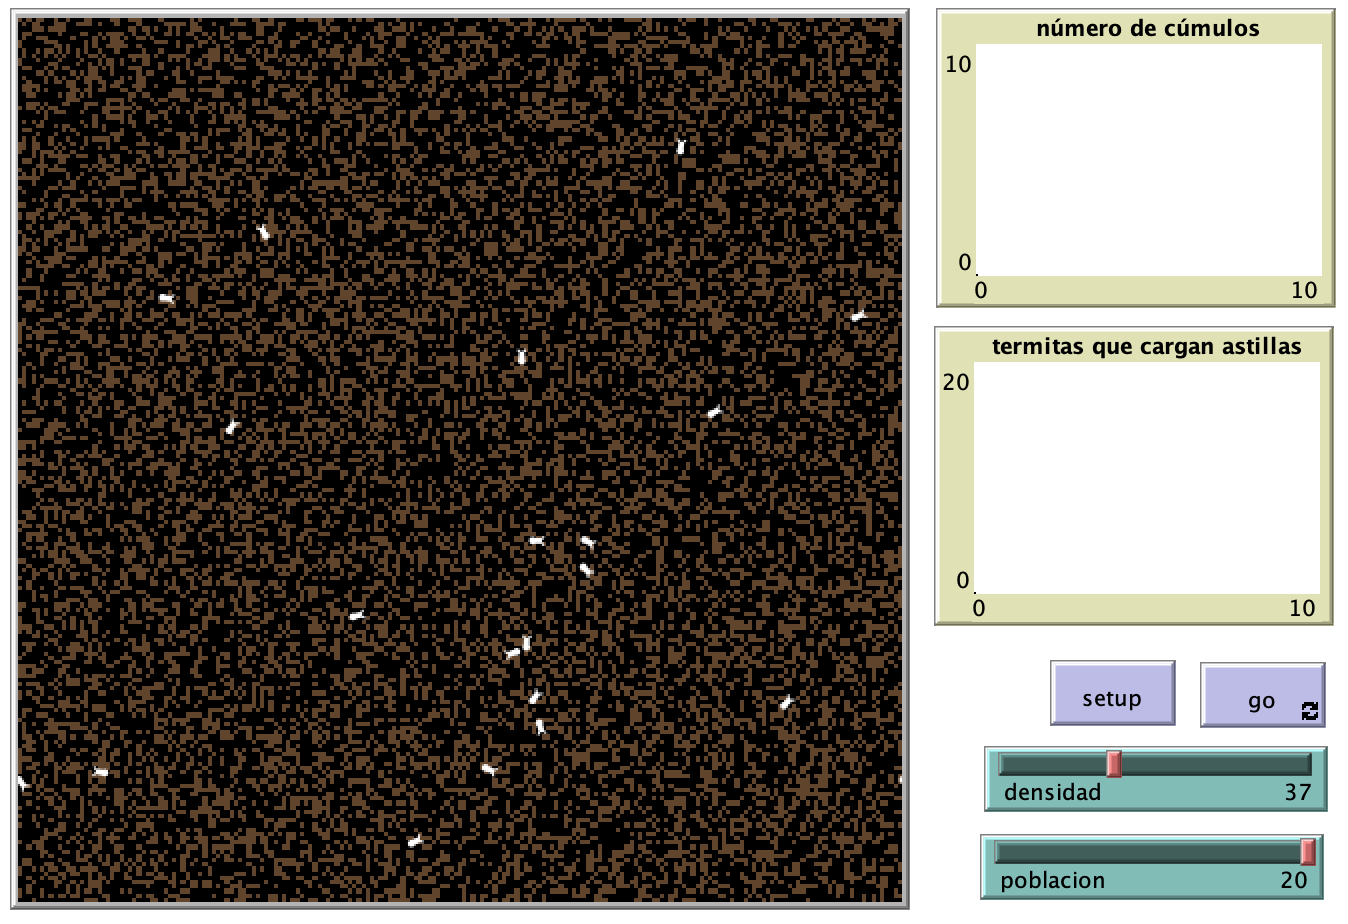
\includegraphics[width=0.7\textwidth]{resources/termitas/06}    
    \caption{Implementación de ambas gráficas en el modelo de termitas apiladoras.}
    \label{fig:termitas-dos} 
	\end{figure} 
	
	
	
	\begin{itemize}
		\item el número de cúmulos en función del tiempo
		
		Se define una variable global \textbf{cumulos}, dentro de la función \textbf{go} se incrementa una unidad a esta variable siempre y cuando se cumpla la siguiente propiedad:
		
		\begin{verbatim}
ask patches [
	if tipo != 0 and visitado = false [
        recorrer-cumulo
        set cumulos cumulos + 1
    ]
]
		\end{verbatim}
		
		En \textbf{recorrer-cumulo} si el patch tiene madera y aún no ha sido visitado entocnes el patch se etiqueta como verdadero. Dada una vecindad de ocho, si uno de los patch tiene presencia de madera y no ha sido visitado entonces continúa (Fig. \ref{fig:001}).
		
	\begin{figure}[H]
    \centering
    \begin{tabular}{ccccc}
        \setlength{\epsfxsize}{0.50\hsize} 
        \subfigure[]{\epsfbox{resources/termitas/07}} & 
        \setlength{\epsfxsize}{0.50\hsize} 
        \subfigure[]{\epsfbox{resources/termitas/08}} 
 
    \end{tabular}
    \vspace{-10pt}
    \caption{(a) Comportamiento de la gráfica en 78,100 ticks cuando el valor de densidad es igual 37 y la población es 20. (b) cómo está implementado el plot.}
    \label{fig:001}
	\end{figure}
		
		\item el número de termitas que están cargando astillas

		Dentro de la función buscar madera los agentes cambian su color a naranja, esto sirve para graficar el número de termitas cargando astillas (Fig. \ref{fig:002}), basta con modificar el valor de la pluma de la gráfica de la siguiente manera:
		\begin{verbatim}
			plot count turtles with [color = orange]
		\end{verbatim}
		
			\begin{figure}[H]
    \centering
    \begin{tabular}{ccccc}
        \setlength{\epsfxsize}{0.50\hsize} 
        \subfigure[]{\epsfbox{resources/termitas/09}} & 
        \setlength{\epsfxsize}{0.50\hsize} 
        \subfigure[]{\epsfbox{resources/termitas/10}} 
 
    \end{tabular}
    \vspace{-10pt}
    \caption{(a) Comportamiento de la gráfica en 78,100 ticks cuando el valor de densidad es igual 37 y la población es 20. (b) cómo está implementado el plot.}
    \label{fig:002}
	\end{figure}
	
	\end{itemize}
	
	\item Extender el modelo considerando dos tipos de astillas de madera (por ejemplo, amarillas y cafés). La termita deja y recoge la astilla a partir del color del cúmulo. ¿cuántas pilas de astillas quedan al final? 
	
	Se modifica la función que asigna el color a los agentes, cuando es de tipo 1 es color café y si es 2 entonces es amarillo, quedaría de la siguiente manera:
	
\begin{verbatim}
to colorea
  if tipo = 1 [set pcolor 33]  
  if tipo = 2 [set pcolor yellow] 
end
\end{verbatim}

Y para la asignación se genera un número aleatorio dentro del setup:

\begin{verbatim}
	set tipo random 3;
\end{verbatim}

Dentro de buscar-madera ahora la termita verifica su tipo, la nueva versión de la función:

\begin{verbatim}
to buscar-madera
  ifelse tipo != 0 [
    set carga tipo
    set tipo 0
    set pcolor black
    set color orange
    forward 10
    set estadoActual 1
  ][
    caminata-aleatoria
  ]
end\end{verbatim}

En la siguiente página de exhibe una ejecución completa del programa, mostrando su historial en doce momentos diferentes donde el valor de densidad es igual a 30 y su población es 10; haciendo un conteo de las pilas de astillas quedaron en total 20. Esta extensión se puede consultar en el archivo 'Termitas-03.nlogo'. 


\begin{figure}
    \centering
    \begin{tabular}{ccc}
        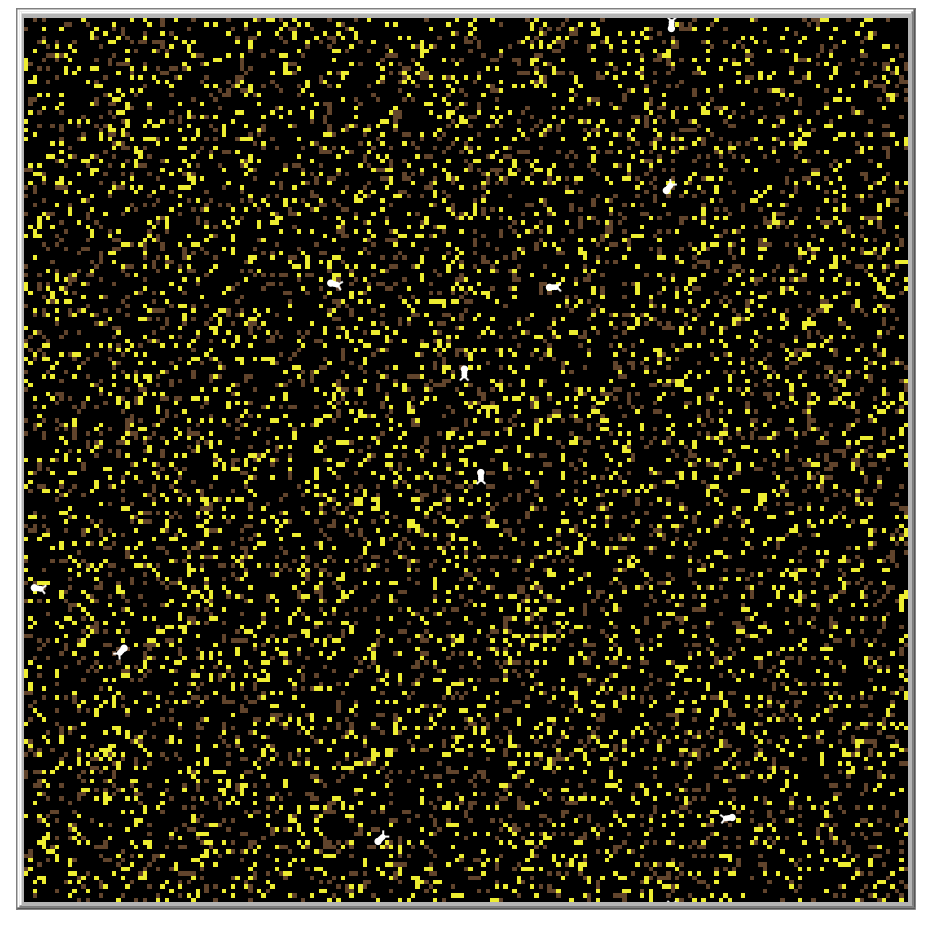
\includegraphics[width=0.3\hsize]{resources/termitas/11} &
        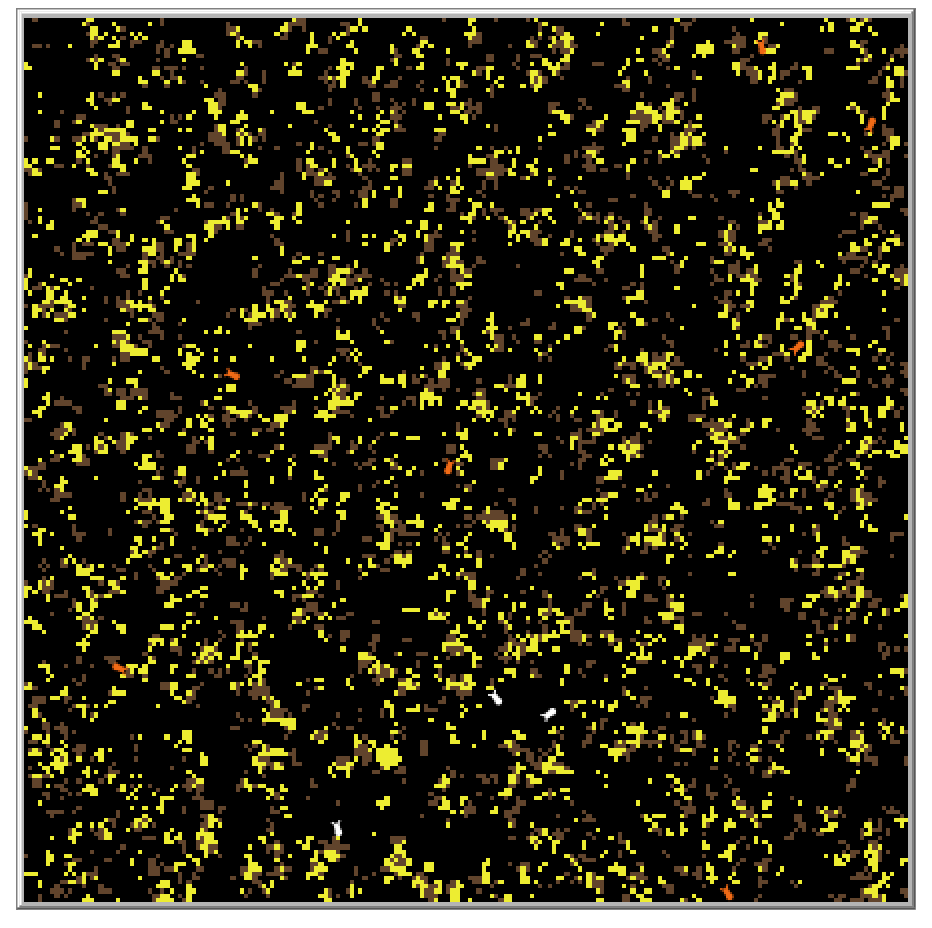
\includegraphics[width=0.3\hsize]{resources/termitas/12} &
        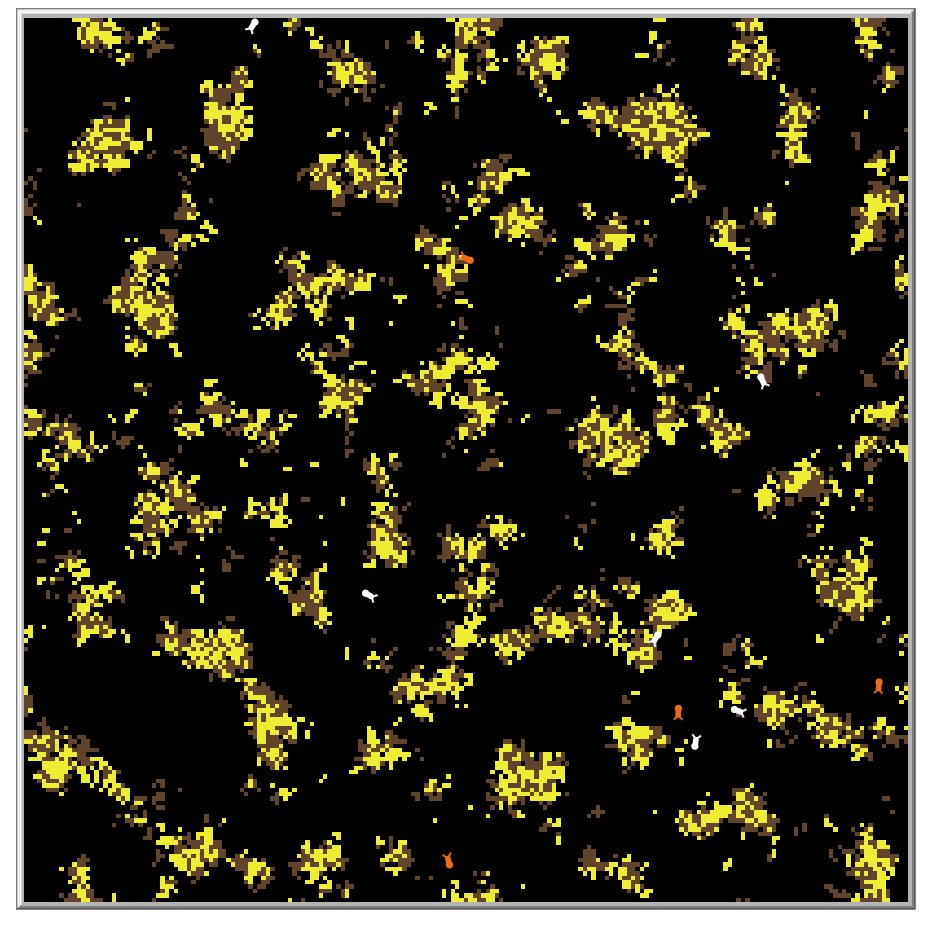
\includegraphics[width=0.3\hsize]{resources/termitas/13} \\
        
        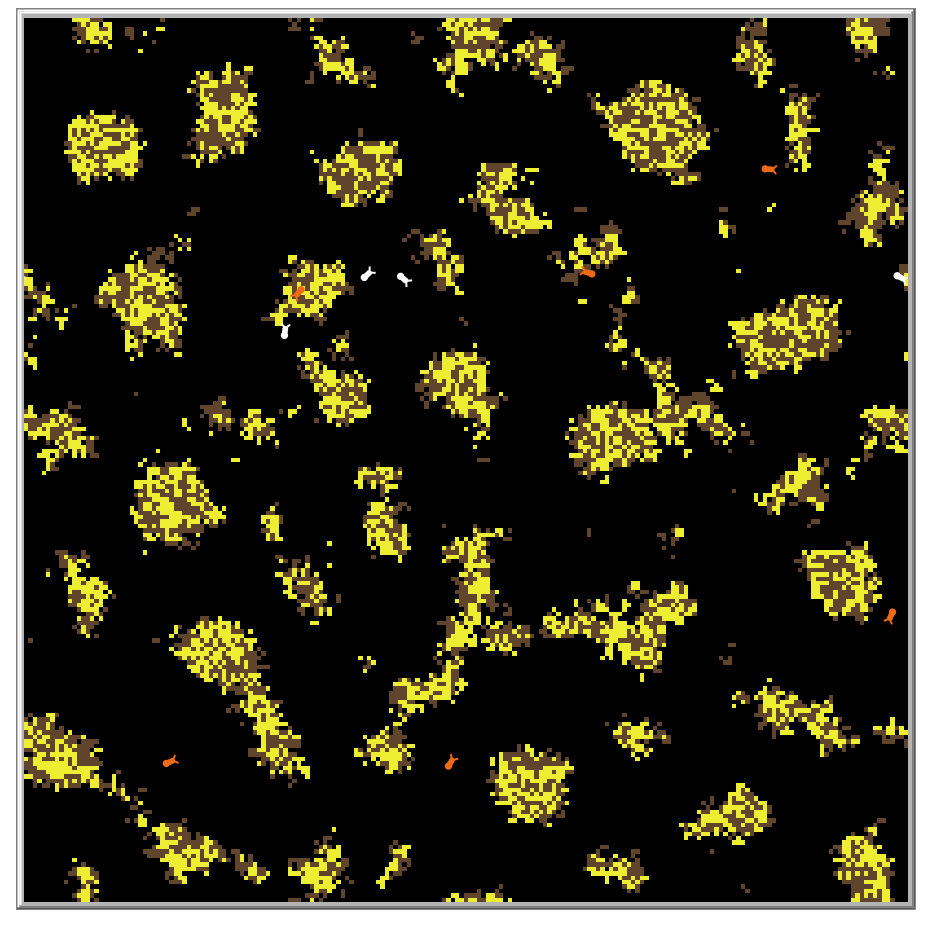
\includegraphics[width=0.3\hsize]{resources/termitas/14} &
        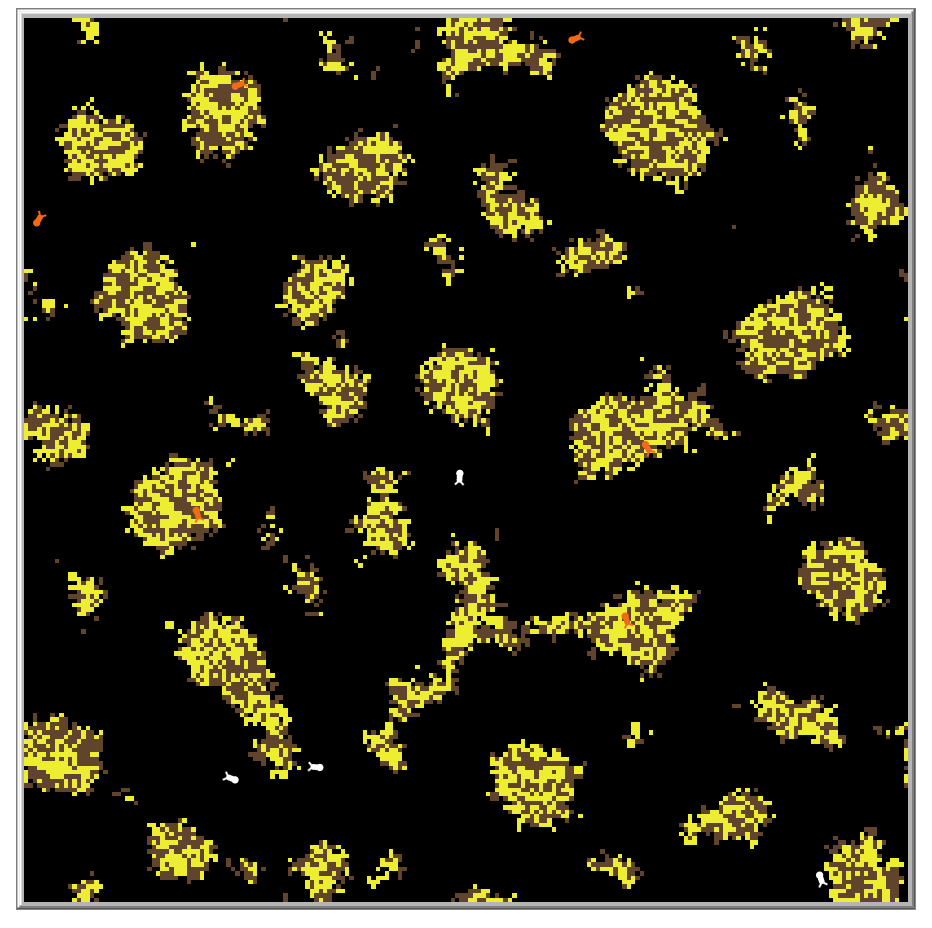
\includegraphics[width=0.3\hsize]{resources/termitas/15} &
        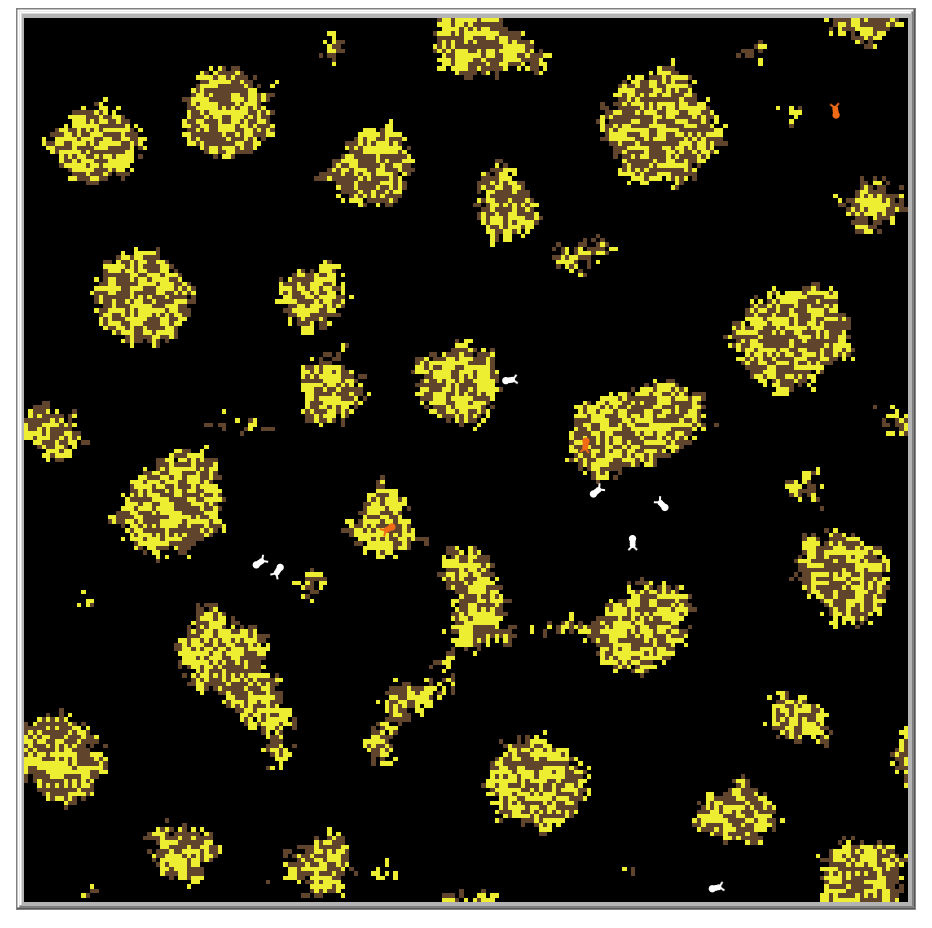
\includegraphics[width=0.3\hsize]{resources/termitas/16} \\
        
        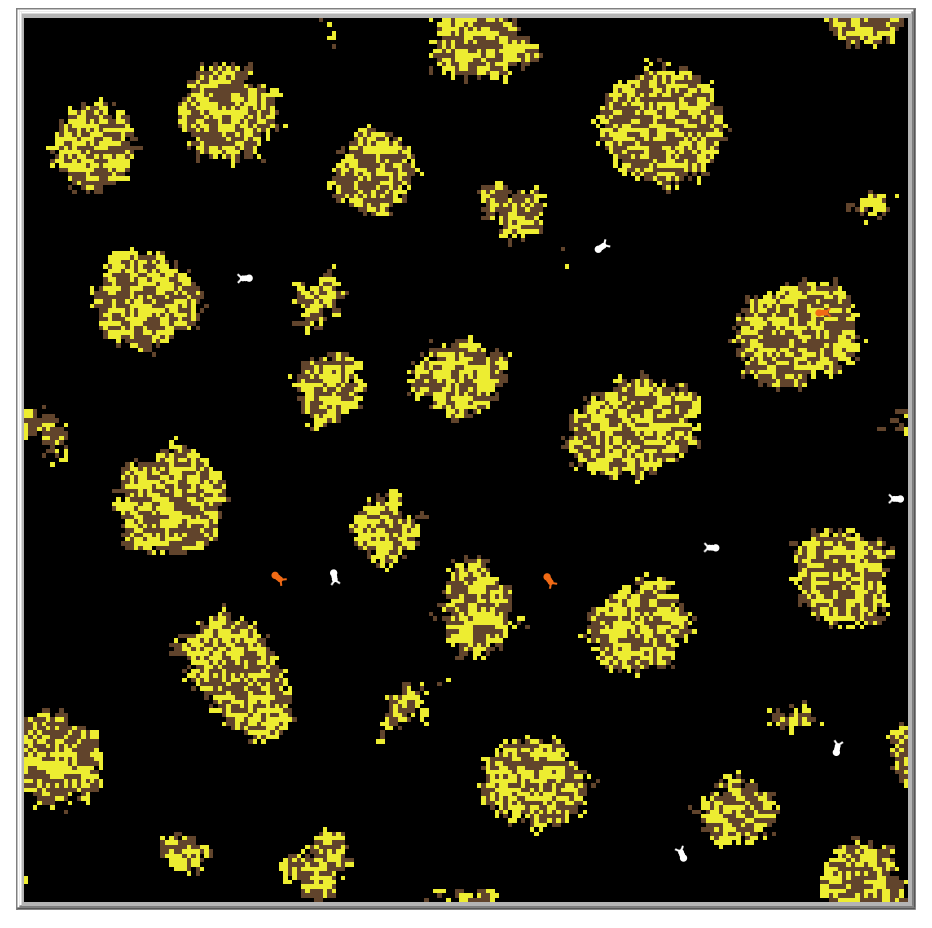
\includegraphics[width=0.3\hsize]{resources/termitas/17} &
        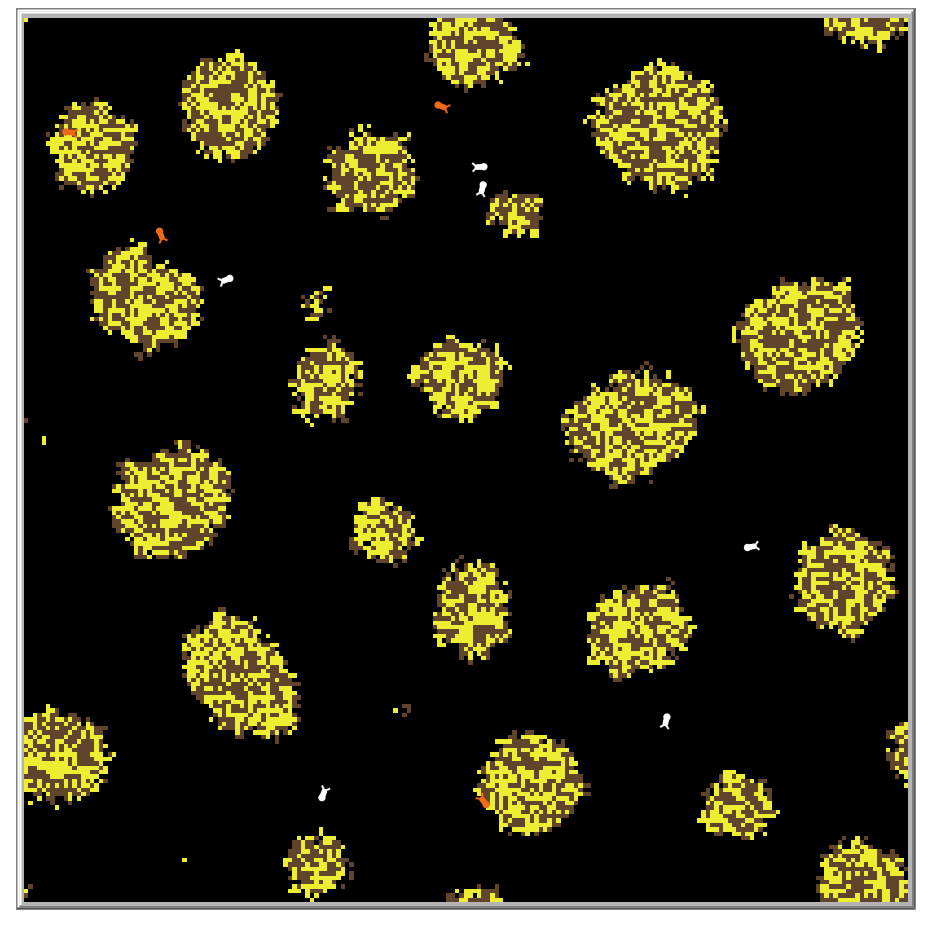
\includegraphics[width=0.3\hsize]{resources/termitas/18} &
        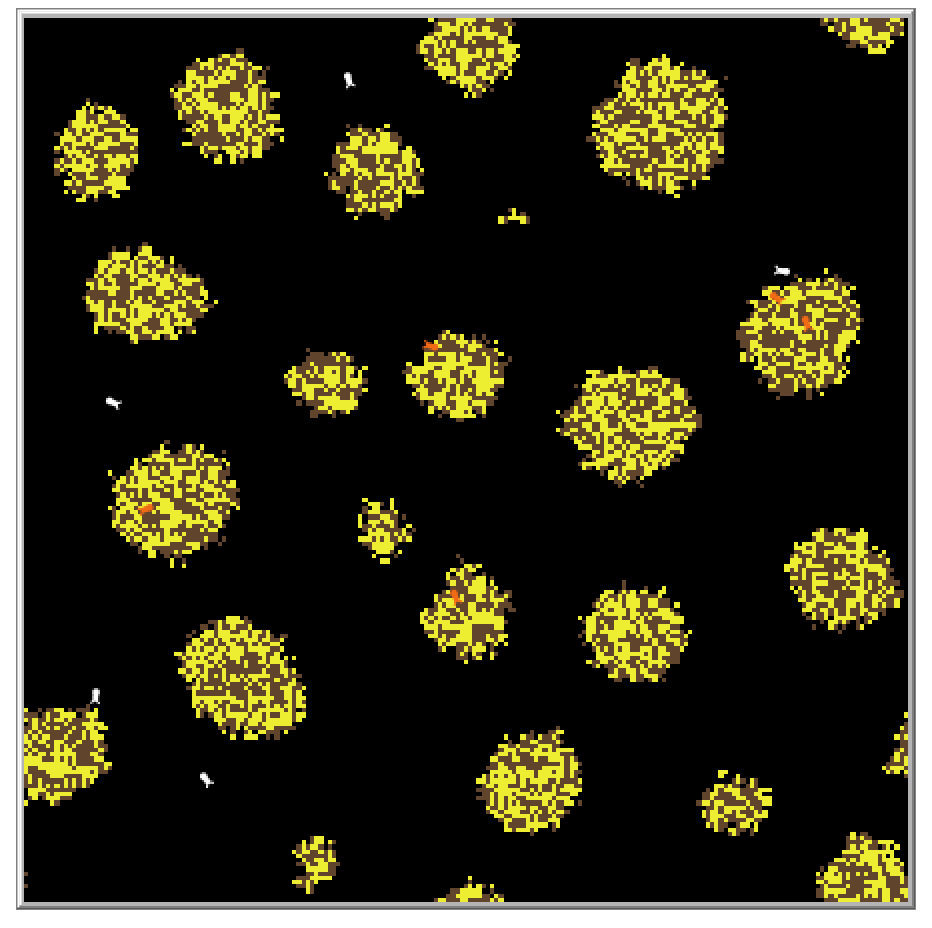
\includegraphics[width=0.3\hsize]{resources/termitas/19} \\
        
        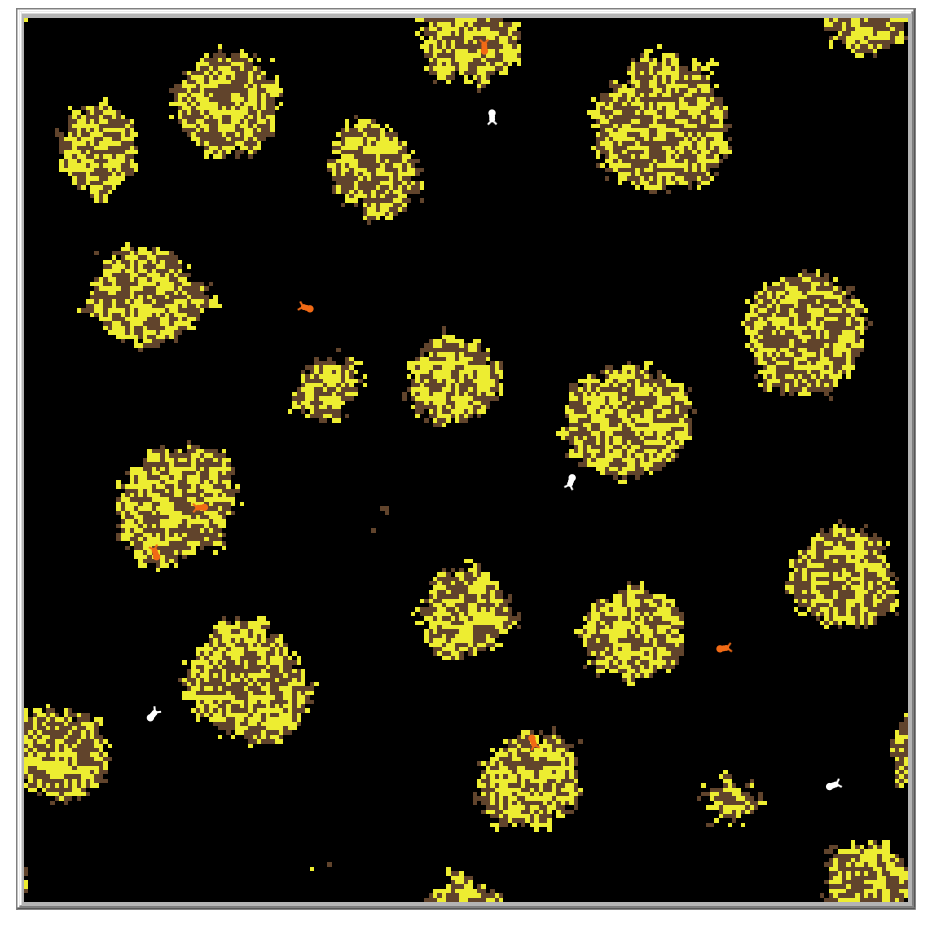
\includegraphics[width=0.3\hsize]{resources/termitas/20} &
        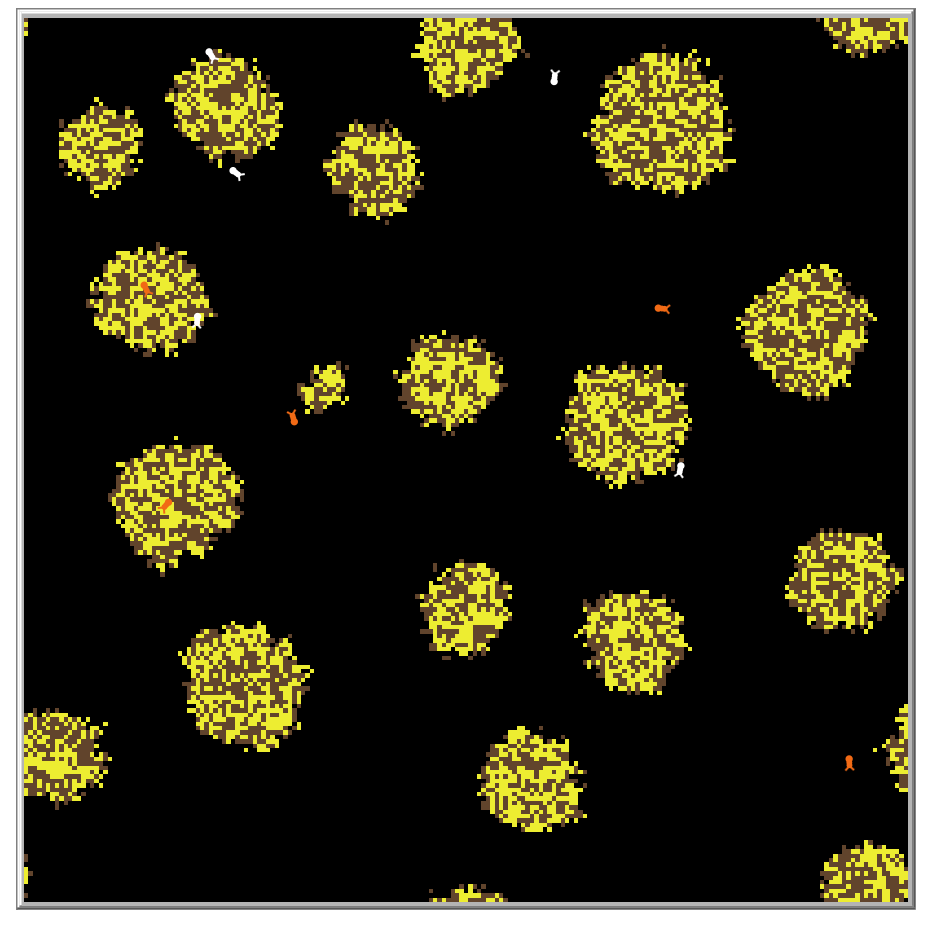
\includegraphics[width=0.3\hsize]{resources/termitas/21} &
        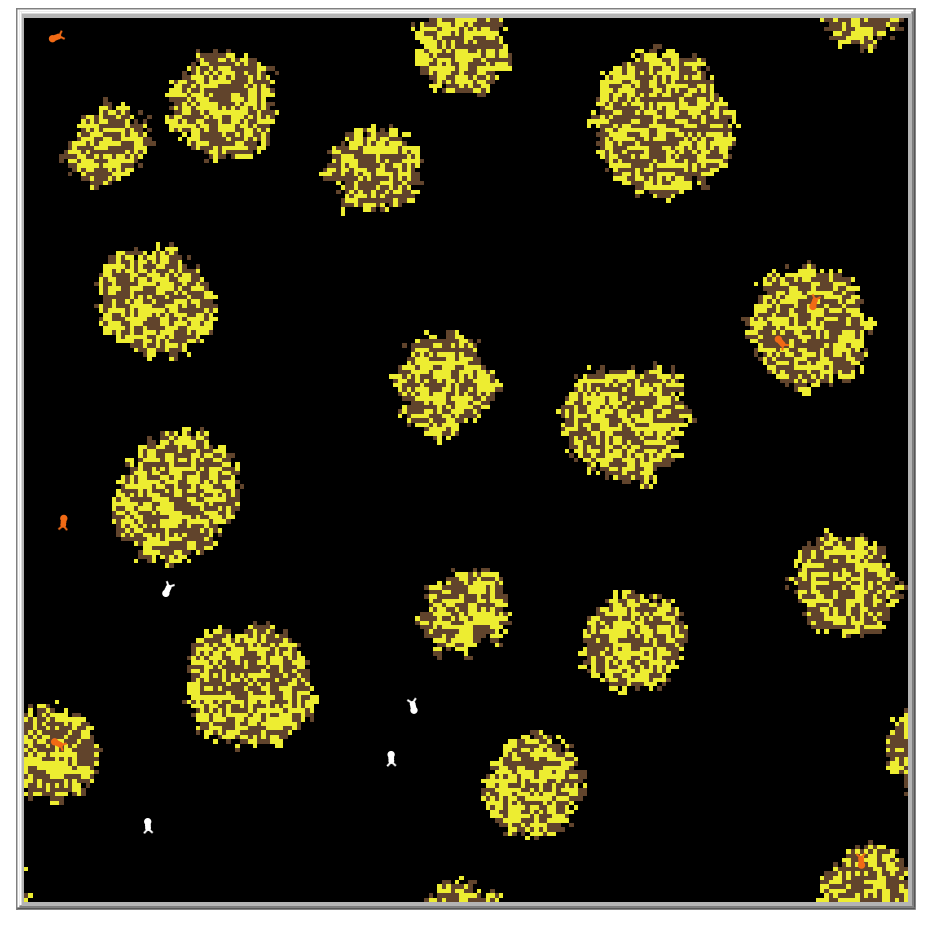
\includegraphics[width=0.3\hsize]{resources/termitas/22} \\
    \end{tabular}
\end{figure}


	
	
	
		
	

\end{enumerate}